% Author: Malte, DE7LMS
% Modifier: Dr. Matthias Jung, DL9MJ
% Modified: Kreuz-Yagi / cross yagi
% Year: 2026

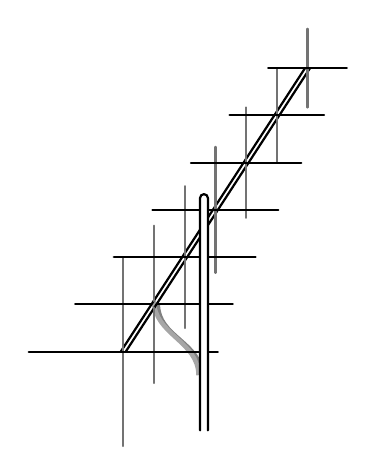
\begin{tikzpicture}[
  thick,
  x={(1cm,0)},
  y={(2.6mm,4mm)},
  z=({0,1cm}),
  line cap=round
]

  \def\s{1.5}
  \def\gap{0.04}

  % styles for the two polarisations
  \tikzset{
    hpol/.style={black},
    vpol/.style={black!55}
  }

  % helper macros
  \def\elementH#1#2{%
    \draw[hpol] (-#1,#2*\s,0) -- (#1,#2*\s,0);
  }

  \def\elementV#1#2{%
    \draw[vpol] (0,#2*\s,-#1) -- (0,#2*\s,#1);
  }

  \def\drivenH#1#2{%
    \draw[hpol] (\gap,#2*\s,0) -- (#1,#2*\s,0);
    \draw[hpol] (-\gap,#2*\s,0) -- (-#1,#2*\s,0);
  }

  \def\drivenV#1#2{%
    \draw[vpol] (0,#2*\s,\gap) -- (0,#2*\s,#1);
    \draw[vpol] (0,#2*\s,-\gap) -- (0,#2*\s,-#1);
  }

  % cables / feed lines
  \path[gray, ultra thick, line cap=butt]
    (0.02,2.5*\s,-1.8) edge[out=90,in=-90] (0.05,1*\s,0);

  \path[gray!70, ultra thick, line cap=butt]
    (-0.02,2.5*\s,-1.8) edge[out=90,in=-90] (0,1*\s,0.05);

  % boom
  \draw[xshift=-0.9pt] (0,0,0) -- (0,9,0);
  \draw[xshift=0.9pt]  (0,0,0) -- (0,9,0);

  % vertical-polarised system, drawn first / slightly lighter
  % reflector
  \elementV{1.2}{0}

  % driven element
  \drivenV{1.0}{1}

  % directors
  \foreach \d/\y in {0.9/2,0.8/3,0.7/4,0.6/5,0.5/6} {
    \elementV{\d}{\y}
  }

  % horizontal-polarised system
  % reflector
  \elementH{1.2}{0}

  % driven element
  \drivenH{1.0}{1}

  % directors
  \foreach \d/\y in {0.9/2,0.8/3,0.7/4,0.6/5,0.5/6} {
    \elementH{\d}{\y}
  }

  % pole
  \draw[rounded corners=.5mm, fill=white]
    (0,2.5*\s,-2.5) -- ++(0,0,3) -- ++(.1,0,0) -- ++(0,0,-3);

\end{tikzpicture}